\appendix
\chapter{Primer apéndice}
\section{Prueba de independencia Chi-Cuadrado de Pearson}
La prueba de independencia Chi-Cuadrado o ji-Cuadrado, nos permite determinar si existe una relación entre dos variables categóricas. Es necesario resaltar que esta prueba nos indica si existe o no una relación entre las variables, pero no indica el grado o el tipo de relación; es decir, no indica el porcentaje de influencia de una variable sobre la otra o la variable que causa la influencia.
\vskip 0.5cm
Para comprender mejor este tema es necesario recordar cuales son los eventos independientes y cuales los dependientes.
\vskip 0.5cm
“Dos eventos aleatorios, $A$ y $B$, son eventos independientes si la probabilidad de un evento no está afectada por la ocurrencia del otro evento; por lo tanto, $p(A) = p(A \mid B)$.”
\vskip 0.5cm
“Dos eventos aleatorios, $A$ y $B$, son eventos dependientes si la probabilidad de un evento está afectada por la ocurrencia del otro; por lo tanto, $p(A) \neq p(A \mid B)$.”
\vskip 0.5cm
Una prueba de independencia usa la pregunta de si la ocurrencia del evento $X$ es independiente a la ocurrencia del evento $Y$, por lo que el planteamiento de las hipótesis para esta prueba de independencia es:
\begin{enumerate}
\item[-]$H_{0}$: La ocurrencia del evento $X$ es independiente del evento $Y$.
\item[-]$H_{1}$: La ocurrencia del evento $X$ no es independiente del evento $Y$.
\end{enumerate}
En las pruebas de independencia se utiliza el formato de la tabla de contingencia, y por esa razón a veces se le llama \textit{prueba de tabla de contingencia}, o \textit{prueba con tabla de contingencia}.
\vskip 0.5cm
Una tabla que clasifica datos de acuerdo a dos o más categorías, relacionados con cada una de las variables cualitativas, que pueden ser o no estadísticamente independientes, se llama \textit{tabla de contingencia}. Dicha tabla muestra todas las posibles combinaciones de categorías, o contingencias, que explican su nombre.
\vskip 0.5cm
A la suma de todas las razones que se puedan construir al tomar la diferencia entre cada frecuencia observada y esperada, en una tabla de contingencia, elevándola al cuadrado, y luego dividiendo esta desviación cuadrada entre la frecuencia esperada, se le llama \textit{estadístico ji-cuadrada}.
\vskip 0.5cm
Procedimiento para elaborar una prueba de independencia:
\begin{enumerate}
\item[1.] Obtener la frecuencia observada ($FO$), proveniente de una encuesta, estudio o experimento.
\item[2.] Resumir los datos obtenidos, es decir, la frecuencia observada, en una tabla de contingencia
\item[3.] Calcular la frecuencia esperada (FE), y se calcula con la siguiente formula:
\[ FE = \frac{(Total Columna)(Total Renglon)}{Gran Total} \]
\item[4.] Determinar el nivel de significancia ($\alpha$), y los grados de libertad, con la siguiente formula:
\[ gl = (\#renglones)(\#columnas) \]
\item[5.] Plantear las hipótesis.
\[ H_{0}: independencia \]
\[ H_{1}: dependencia \]
\item[6.] Construir las áreas de aceptación y rechazo.
\item[7.] Calcular ji-Cuadrada $X^{2}$
\[ X^{2}_{exp} = \sum_{i=1}^{n} \frac{(FO - FE)^2}{FE} \]
\item[8.] Tomar una decisión y emitir una conclusión en términos del problema.
\end{enumerate}

A continuación, mostraremos algunos valores de la Tabla de Distribución Chi Cuadrado, donde $v$ representa a los grados de libertad ($gl$) y $p$ la probabilidad de encontrar un valor mayor o igual que el Chi-Cuadrado tabulado, también llamado como nivel de significancia ($\alpha$).


\begin{center}
\begin{table}[h!]
\centering
\vskip -0.2cm
\caption{\small{Tabla de distribución Chi-Cuadrado.}}
\label{table:tablaA.1}
\begin{tabular}{c}
\begin{minipage}{.9\textwidth}
\begin{center}
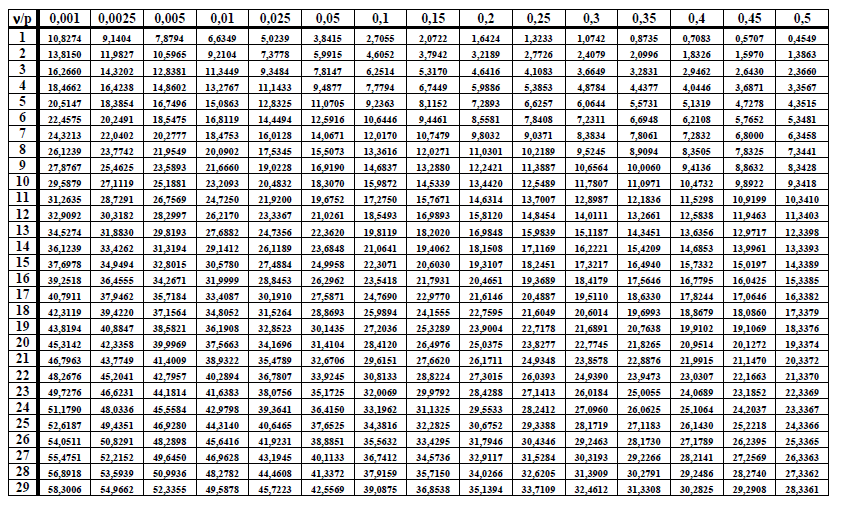
\includegraphics[width=1\textwidth]{Imagenes/Apendice/image001}
\end{center}
\end{minipage}
\end{tabular}
\begin{center}
\vskip 0.2cm
{\small{Fuente: \cite{eyra}}}
\end{center}
\end{table}
\end{center}